\pagestyle{aaron}
\section{Modellierung des Schwungrad-Pendels} \label{sec:Modellierung}

Der folgende Abschnitt beschäftigt sich mit der Modellierung des Schwungrad-Pendels inklusive des treibenden Gleichstrommotors.

\subsection{Modellierung des Gleichstrommotors}

\begin{figure}[H]
    \centering
    \fbox{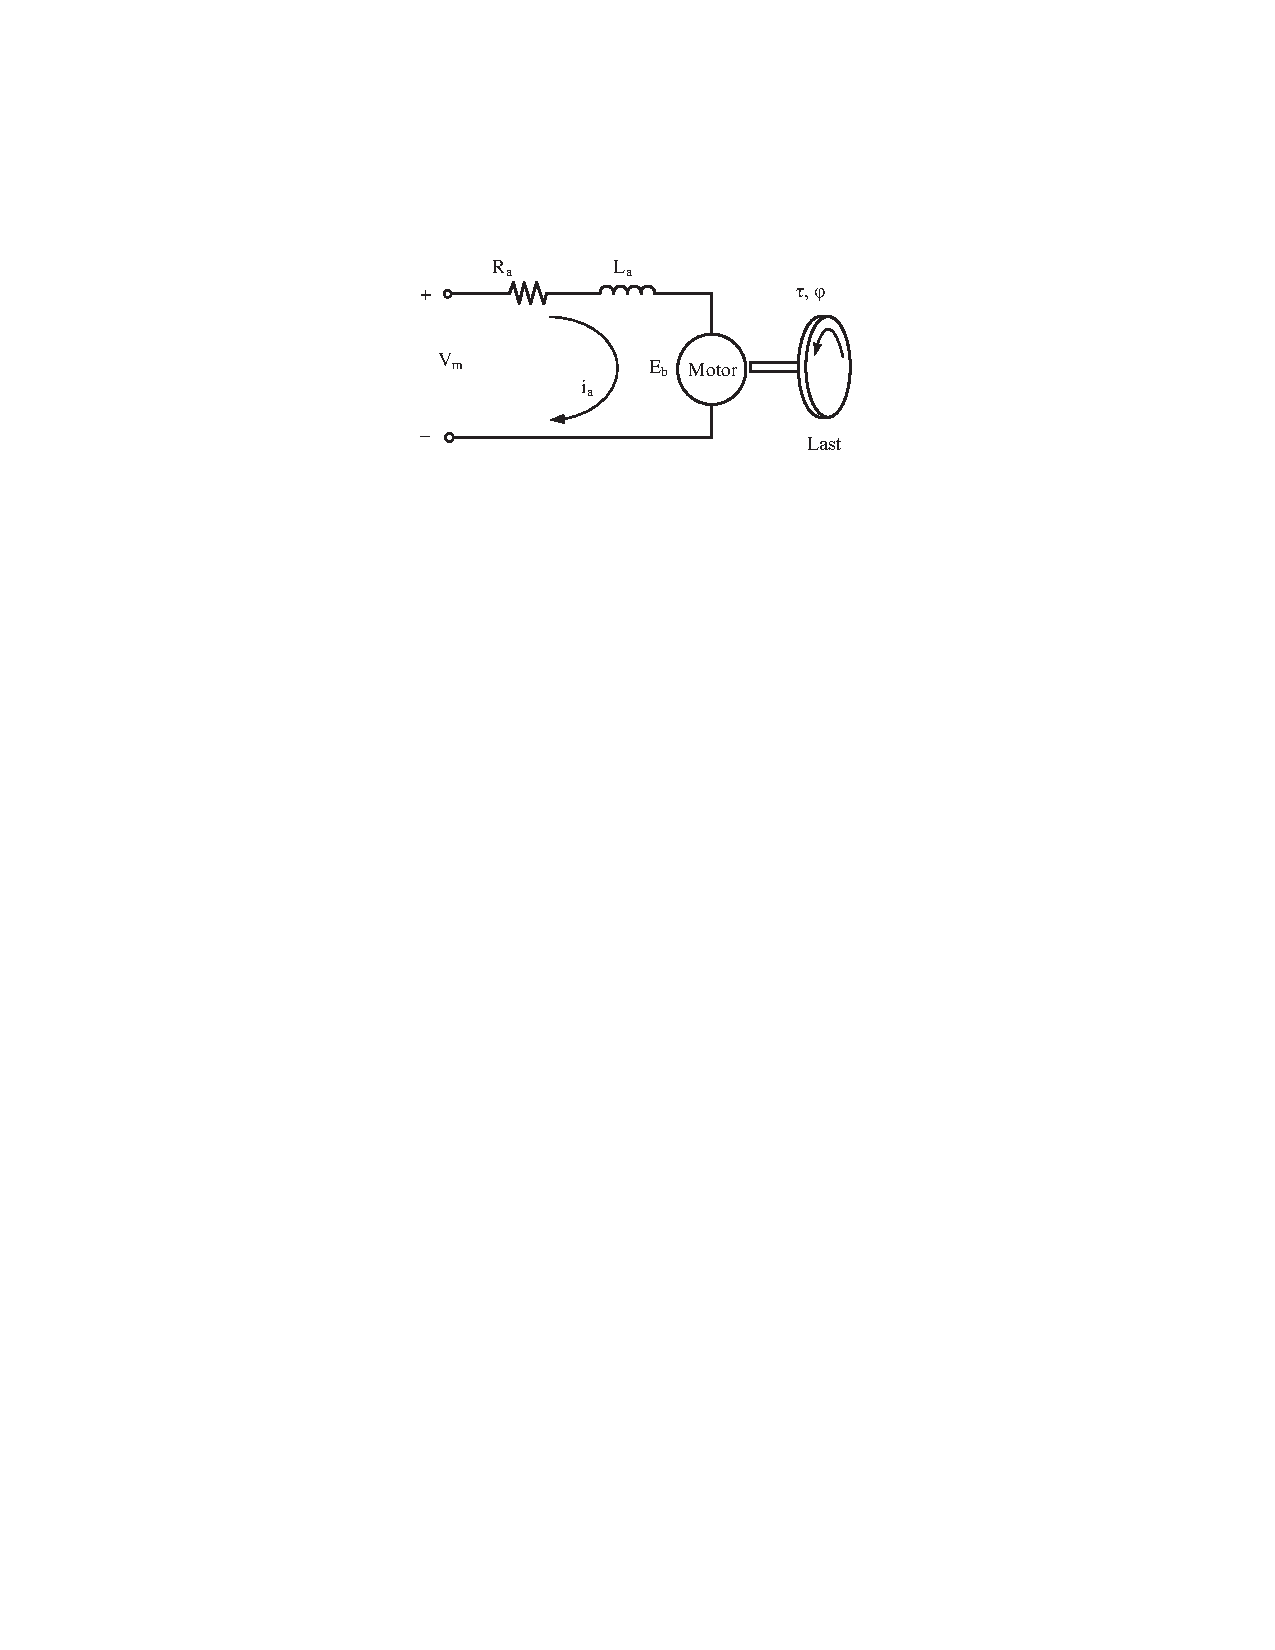
\includegraphics[width=0.6\textwidth]{Bilder/2_modellierung/Ersatzschaltbild.pdf}}
    \caption[Ersatzschaltbild Gleichstrommotor]{Ersatzschaltbild des Gleichstrommotors am Schwungrad-Pendel}
    \label{fig:Bild2.1}
\end{figure}

\autoref{fig:Bild2.1} zeigt das Ersatzschaltbild des Gleichstrommotors am Schwungrad-Pendel. Das zweite Kirchhoff'sche Gesetzt ergibt folgende Gleichung:

\begin{equation} \label{eq:Gleichung2.1}
    V_{\mathrm{m}} = i_{\mathrm{a}} R_{\mathrm{a}} + L_{\mathrm{a}} \frac{di_{\mathrm{a}}}{dt} + E_{\mathrm{b}}
\end{equation}
\newline
Die gegenelektromotorische Kraft (EMK) hängt von der Winkelgeschwindigkeit $\dot\varphi$ und der Gegen-EMK-Konstante $K_{\mathrm{b}}$ wie folgt ab:

\begin{equation} \label{eq:Gleichung2.2}
    E_{\mathrm{b}} = K_{\mathrm{b}} \dot\varphi
\end{equation}
\newline
Angenommen die Wirkung der Induktivität ist sehr klein ($L_{\mathrm{a}} \ll R_{\mathrm{a}}$), \autoref{eq:Gleichung2.1} ergibt sich zu

\begin{equation} \label{eq:Gleichung2.3}
    i_{\mathrm{a}} = \frac{V_{\mathrm{m}} - K_{\mathrm{b}} \dot\varphi}{R_{\mathrm{a}}}.
\end{equation}
\newline
Das Motordremoment $\tau$ ist mit dem Ankerstrom $i_{\mathrm{a}}$ durch eine Motordrehmomentkonstante $K_{\mathrm{t}}$ verbunden. Die Modellgleichung des Gleichstrommotors ergibt sich somit zu:

\begin{equation} \label{eq:Gleichung2.4}
    \boxed{\tau = K_{\mathrm{t}} i_{\mathrm{a}} = K_{\mathrm{t}} \frac{V_{\mathrm{m}} - K_{\mathrm{b}} \dot\varphi}{R_{\mathrm{a}}}}
\end{equation}

\subsection{Modellierung des Schwungrad-Pendels}

Zur Modellierung des Pendels wurde der Langrange-Ansatz gewählt, um die Bewegungsgleichungen des Pendels herzuleiten.
 
\subsubsection{Lagrange Ansatz}

Die nachfolgende Gleichung zeigt den \textbf{Lagrange Ansatz} unter Berücksichtigung der \textbf{dissipativen Funktion}. Diese besagt in Erweiterung zu der Lagrange-Formulierung, dass Energie in einem Vorgang in Wärme umgewandelt wird. Mit Hilfe der dissipativen Funktion können \textbf{Reibungsverluste} bei der Energiemethode nach Lagrange berücksichtigt werden.
\begin{equation} \label{eq:Gleichung2.5}
    \boxed{\frac{d}{dt} \left(\frac{\partial L}{\partial \dot{q_{\mathrm{i}}}}\right) - \frac{\partial L}{\partial q_{\mathrm{i}}} + \frac{\partial D}{\partial \dot{q_{\mathrm{i}}}} = 0}
\end{equation}

\subsubsection{Freiheitsgrade und Zwangsbedingungen}

In \autoref{fig:Bild1.1} sind zwei Teilchen \bzw Massepunkte im $\mathbb{R}^2$ zu erkennen. Zum Einen die des Pendels und zum Anderen die des Schwungrades. Somit gilt grundsätzlich:

\begin{itemize}
    \item 2 Punkte: 4 Freiheitsgrade (FHG)
\end{itemize}

Das Schwungrad-Pendel besitzt jedoch auch zwei Zwangsbedingungen, die wie folgt formuliert werden können:

\begin{itemize}
    \item Das Pendel kann nur um die 0z-Achse rotieren: \\ $z = 0$
    \item Die Masse $m_2$ ist über des Pendel mit dem Aufhängepunkt 0 gekoppelt: \\ $(y_{\mathrm{m_1}} - y_{\mathrm{m_2}})^2 + (x_{\mathrm{m_1}} - x_{\mathrm{m_2}})^2 = l_2^2$
\end{itemize}

Beide Zwangsbedingungen sind holonom-skleronom, da sie als Gleichungen zwischen zwei Koordinaten angegeben werden können und nicht von der Zeit abhängig sind.

Somit bleiben am Ende noch zwei Freiheitsgrade (FHG) übrig.

\subsubsection{Generalisierte Koordinaten}

Aus den verbliebenen Freiheitsgraden werden die generalisierten Koordinaten abgeleitet. Dabei gilt grundsätzlich folgender Zusammenhang im $\mathbb{R}^2$:

\begin{equation} \label{eq:Gleichung2.6}
    \boxed{S = 2n - k}
\end{equation}
\newline
mit $S$ als Anzahl der Freiheitsgrade und somit auch der Anzahl der generalisierten Koordinaten, $n$ der Anzahl der Teilchen und $k$ der Anzahl der holonomen Zwangsbedingungen.\\
Die beiden Generalisierten Koordinaten sind somit:

\begin{itemize}
    \item $q_{\mathrm{1}} = \theta$
    \item $q_{\mathrm{2}} = \varphi$
\end{itemize}

\subsubsection{Berechnung der kinetischen und potentiellen Energie}

Für die Lagrange-Formulierung werden die kinetische und die potentielle Energie des Systems benötigt. Die kinetische Energie setzt sich zusammen aus der translatorischen kinetischen Energie $E_{\mathrm{kin,trans}}$ und der rotatorischen kinetischen Energie $E_{\mathrm{kin,rot}}$. Die Gleichungen sind nachfolgend aufgestellt.

\begin{align} \label{eq:Gleichung2.7}
    \begin{split}
        E_{\mathrm{kin,trans}} &= \frac{1}{2} m_1 (l_1\dot\theta)^2 + \frac{1}{2}m_2 (l_2\dot\theta)^2 \\
        E_{\mathrm{kin,rot}} &= \frac{1}{2} J_1 (\dot\theta)^2 + \frac{1}{2} J_2 (\dot\theta + \dot\varphi)^2
    \end{split}
\end{align}
\newline
Die gesamte \textbf{kinetische Energie des Systems} ist somit:

\begin{empheq}[box=\widefbox]{align} \label{eq:Gleichung2.8}
    \begin{split}
        E_{\mathrm{kin}} &= E_{\mathrm{kin,trans}} + E_{\mathrm{kin,rot}} \\
        E_{\mathrm{kin}} &= \frac{1}{2} \left( m_1 l_1^2 + m_2 l_2^2 + J_1 + J_2 \right) \dot\theta^2 + J_2\dot\theta\dot\varphi + \frac{1}{2} J_2 \dot\varphi^2
    \end{split}
\end{empheq}
\newline
Der Ursprung der potentiellen Energie liegt bei Null. Somit ergibt sich die \textbf{potentielle Energie des Systems} zu:

\begin{equation} \label{eq:Gleichung2.9}
    \boxed{E_{\mathrm{pot}} = \left( m_1 l_1 + m_2 l_2 \right) g\cos (\theta)}
\end{equation}

\subsubsection{Herleitung der Bewegungsgleichungen}

Die \textbf{Lagrange-Funktion} $L$ wird aus der Differenz der kinetischen Energie aus \autoref{eq:Gleichung2.8} und der potentiellen Energie aus \autoref{eq:Gleichung2.9} berechnet.

\begin{empheq}[box=\widefbox]{align} \label{eq:Gleichung2.10}
    \begin{split}
        L &= E_{\mathrm{kin}} - E_{\mathrm{pot}} \\
        L &= \frac{1}{2} \left( m_1 l_1^2 + m_2 l_2^2 + J_1 + J_2 \right) \dot\theta^2 + J_2\dot\theta\dot\varphi + \frac{1}{2} J_2 \dot\varphi^2 - \left( m_1 l_1 + m_2 l_2 \right) g\cos (\theta)
    \end{split}
\end{empheq}
\newline
Die \textbf{dissipative Energie} $D$ ist:

\begin{equation} \label{eq:Gleichung2.11}
    \boxed{D = \frac{1}{2} c_1 \dot\theta^2 + \frac{1}{2} c_2 \dot\varphi^2}
\end{equation}
\newline
Zieht man nun den Ansatz aus \autoref{eq:Gleichung2.5} heran und wendet diesen für die generalisierte Koordinate $\theta$ an, so erhält man die \textbf{Bewegungsgleichung des Schwungrades}:

\begin{equation} \label{eq:Gleichung2.12}
    \boxed{\left( m_1 l_1^2 + m_2 l_2^2 + J_1 + J_2\right) \ddot\theta + J_2\ddot\varphi + c_1\dot\theta - \left( m_1 l_1 + m_2 l_2 \right) g\sin (\theta) = 0}
\end{equation}
\newline
Ebenfalls der Gleiche Ansatz wird nun für die generalisierte Koordinate $\varphi$ angewendet:

\begin{equation} \label{eq:Gleichung2.13}
    J_2 \left( \ddot\theta + \ddot\varphi \right) + c_2 \dot\varphi = \tau
\end{equation}
\newline
Setzt man nun \autoref{eq:Gleichung2.4} in \autoref{eq:Gleichung2.13} ein erhält man die \textbf{Bewegungsgleichung des Pendels}:

\begin{equation} \label{eq:Gleichung2.14}
    \boxed{J_2 \left( \ddot\theta + \ddot\varphi \right) + c_2 \dot\varphi = K_{\mathrm{t}} i_{\mathrm{a}} = K_{\mathrm{t}} \frac{V_{\mathrm{m}} - K_{\mathrm{b}} \dot\varphi}{R_{\mathrm{a}}}}
\end{equation}